% Chapter X

\chapter{The ATLAS Detector} % Chapter title

\label{ch:atlas} % For referencing the chapter elsewhere, use \autoref{ch:name} 

The ATLAS detector circumscribes the \ac{LHC}'s beam pipe, enclosing the collision point with a series of particle detecting layers, aimed at making as many measurements of the particles leaving the collision point as possible. Its goal is to get a precise measurement of all the stable or semi-stable particles flying from proton-proton collisions at its center, allowing analyzers to fully reconstruct the kinematics of the underlying processes.

The ATLAS detector is the largest detector of its kind, measuring 44 m in length and 25 m in height, as seen in \autoref{fig:detector}. The size is mainly determined by the constraints of the \ac{MS}, discussed in \autoref{sec:MS}, which is the largest and outermost subsystem. The \ac{MS} is submerged in a spatially varying magnetic field provided by three toroidal magnets, while the \ac{ID} (\autoref{sec:ID}) is encased by a superconducting solenoid, which provides a uniform 2 T field throughout its volume \cite{PERF-2007-01}.

\begin{centering}
\begin{figure}[bth]
\myfloatalign
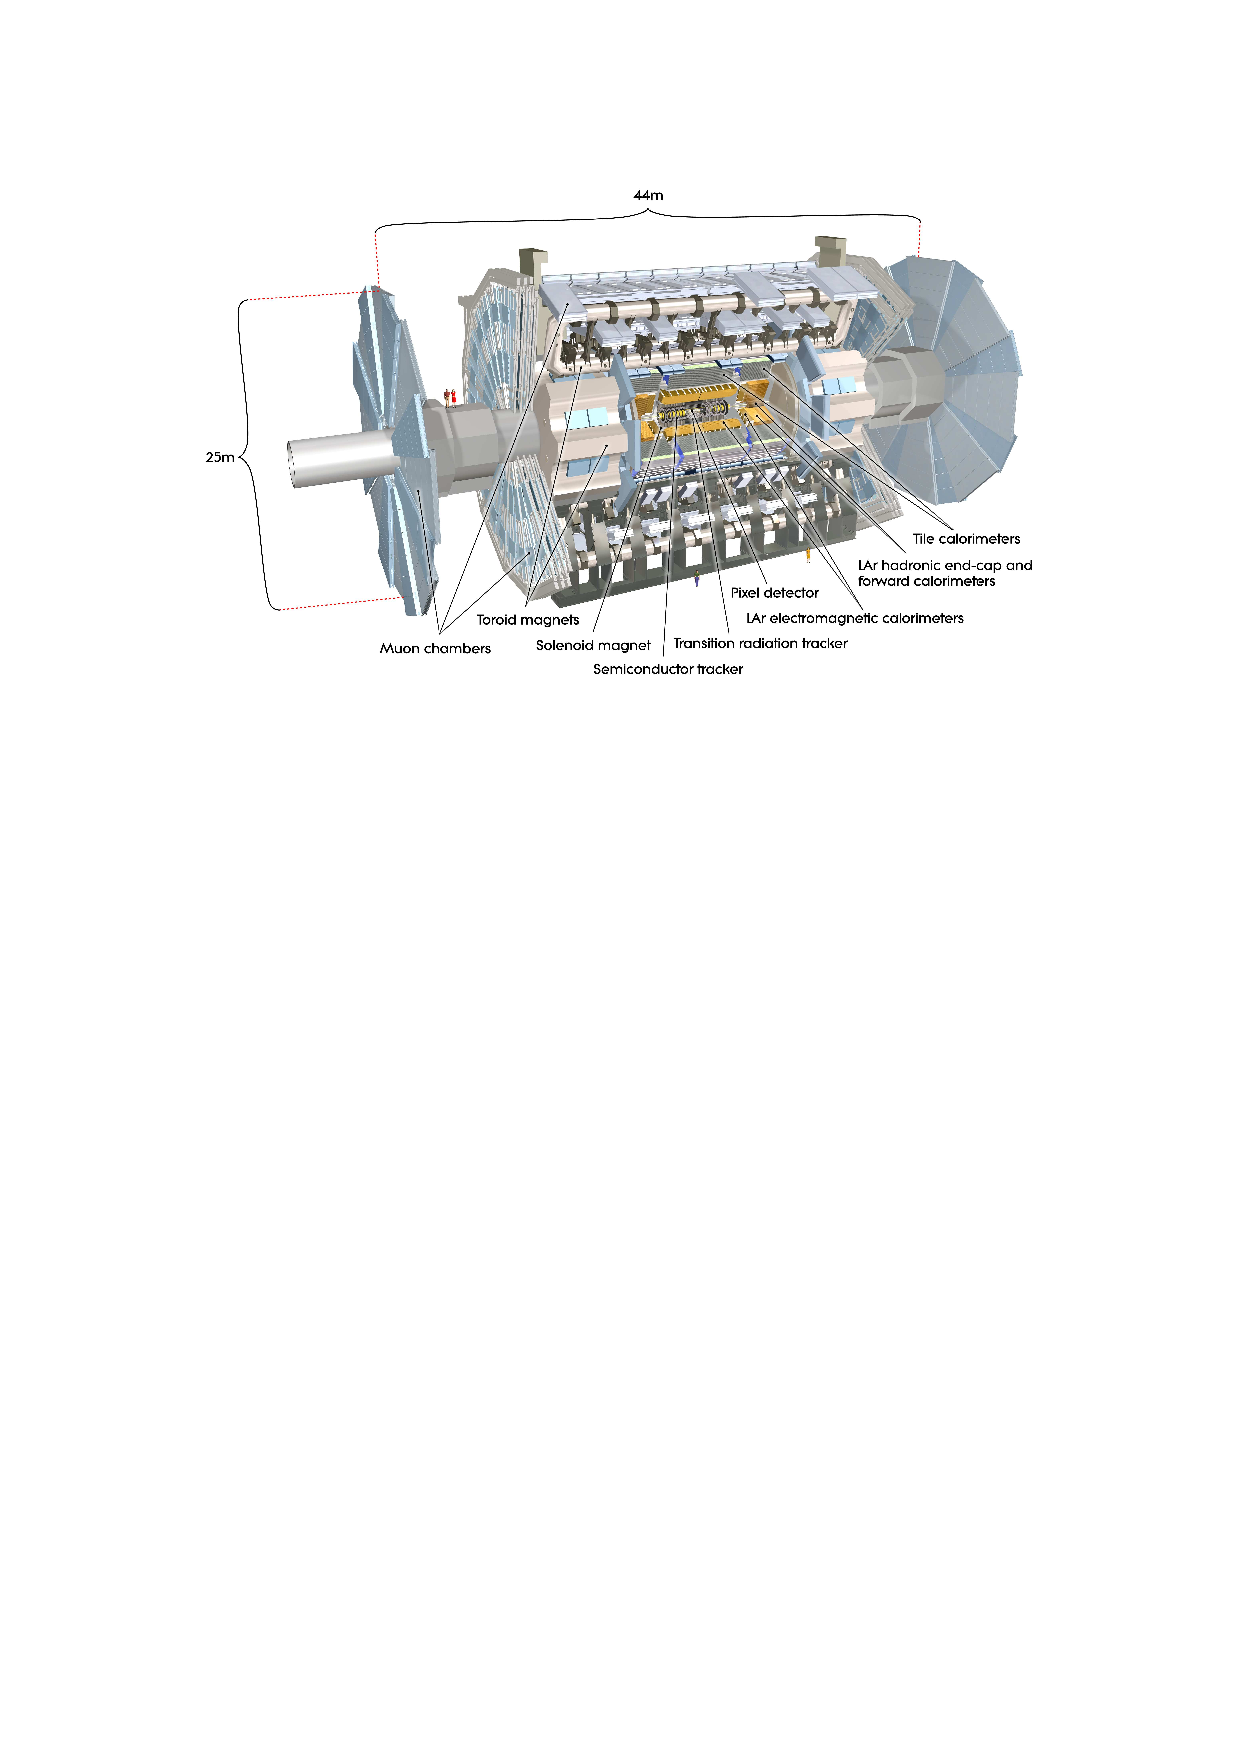
\includegraphics[width=.90\linewidth]{figures/atlas/detector.pdf}
\caption{Diagram of the ATLAS detector, with subsystems and magnets identified.}
\label{fig:detector}
\end{figure}
\end{centering}

\section{Coordinate System Used in the ATLAS Detector}

The ATLAS detector is centered around a the collision point in the beam pipe, and is built radially out from the pipe, maintaining as much rotational symmetry as possible. It is also symmetric in the forward-backward directions. Because of this geometry, a coordinate system using the collision point as the origin is used, with the beam pipe defining the $z$-axis. The positive $x$ direction is defined as pointing to the center of the \ac{LHC} ring, while the positive $y$ direction points upwards. For ease of reference, the side of the detector in the positive-$z$ direction is referred to as the A side, and the other side is referred to as the C side. 

Because of the radial design of the detector, angular coordinates are often used. The azimuthal angle $\phi$ defines the radial distance around the beam pipe and the polar angle $\theta$ defines the angle from the beam axis ($z$). However, a transformation of the polar angle called pseudorapidity ($\eta$) is used more often, and is defined as 

\begin{equation}
\eta = - ln [ tan \frac{\theta}{2} ]. 
\end{equation}

Building on this variable definition, distance between objects is typically defined as

\begin{equation}
\Delta R = \sqrt{\Delta\eta^2 + \Delta\phi^2}. 
\end{equation}

Often variables are defined purely in the transverse plane, which is indicated by a subscripted $T$, as in $p_T$, which gives an object's transverse momentum. Another common usage is $E_T^{miss}$, which gives the negative vectorial sum of the energy in an event. 

%------------------------------------------------

\section{The Inner Detector}
\label{sec:ID}

One goal of the ATLAS detector is to produce tracks, predictions of the paths particles take as they travel through the detector. Collisions in the detector produce about 1000 particles, so identifying and differentiating all these tracks is both a hardware and a computational challenge. The \ac{ID}, also called the Tracker, is responsible for providing high enough resolution measurements that each of these tracks and its precise position can be recorded. This tracking system consists of three subdetectors which each produce electrical responses to charged particles passing through their active material. Each of these signals is called a hit. ATLAS tracking software considers all these hits and forms tracks, with the goal of minimizing fake tracks due to random noise. Some details of this process is discussed at length in \autoref{sec:NN}. The full \ac{ID} can be seen in \autoref{fig:ID}, while a schematic in \autoref{fig:IDeta} demonstrates the $\eta$ coverage of each detector.

\begin{centering}
\begin{figure}[bth]
\myfloatalign
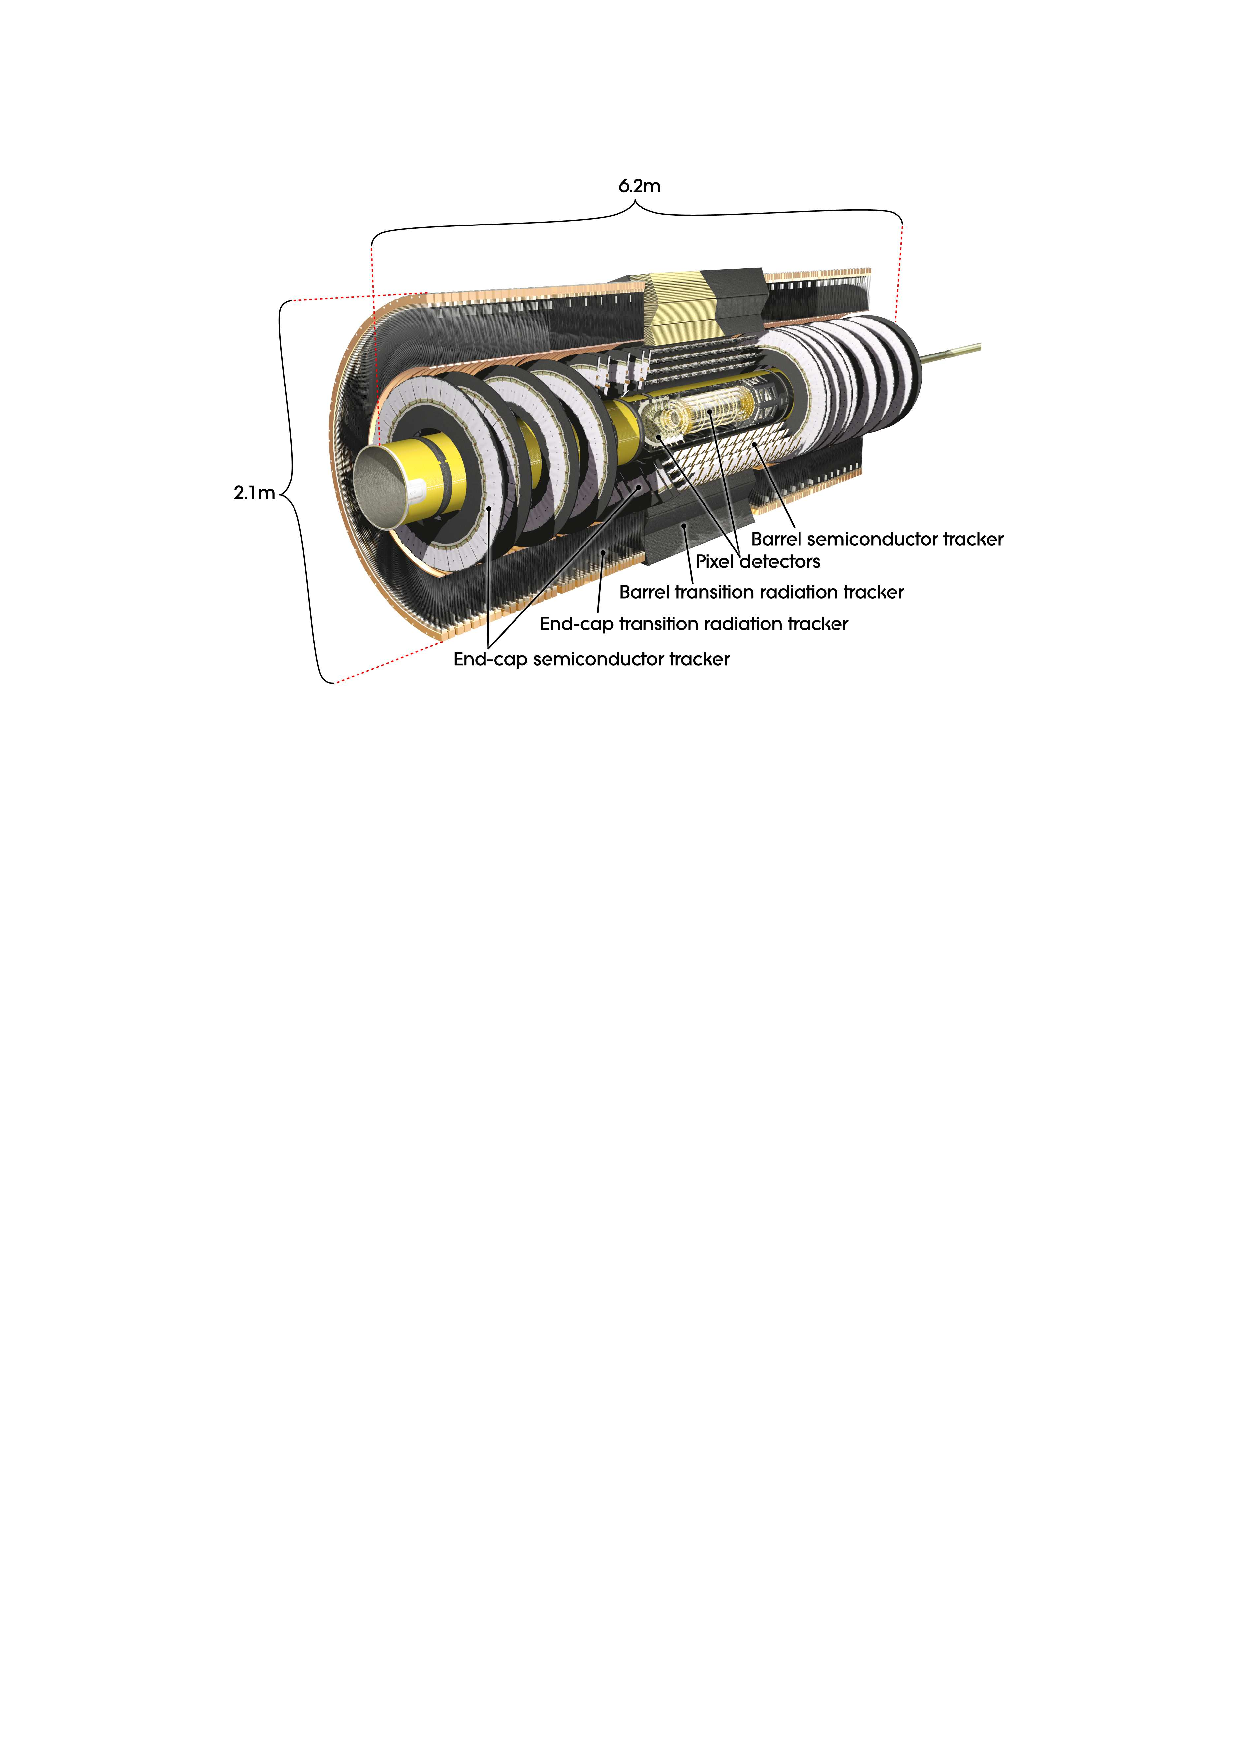
\includegraphics[width=.90\linewidth]{figures/atlas/innerdetector.pdf}
\caption{Diagram of the ATLAS Inner Detector, containing the Pixel, SCT, and TRT subsystems.}
\label{fig:ID}
\end{figure}
\end{centering}

\begin{centering}
\begin{figure}[bth]
\myfloatalign
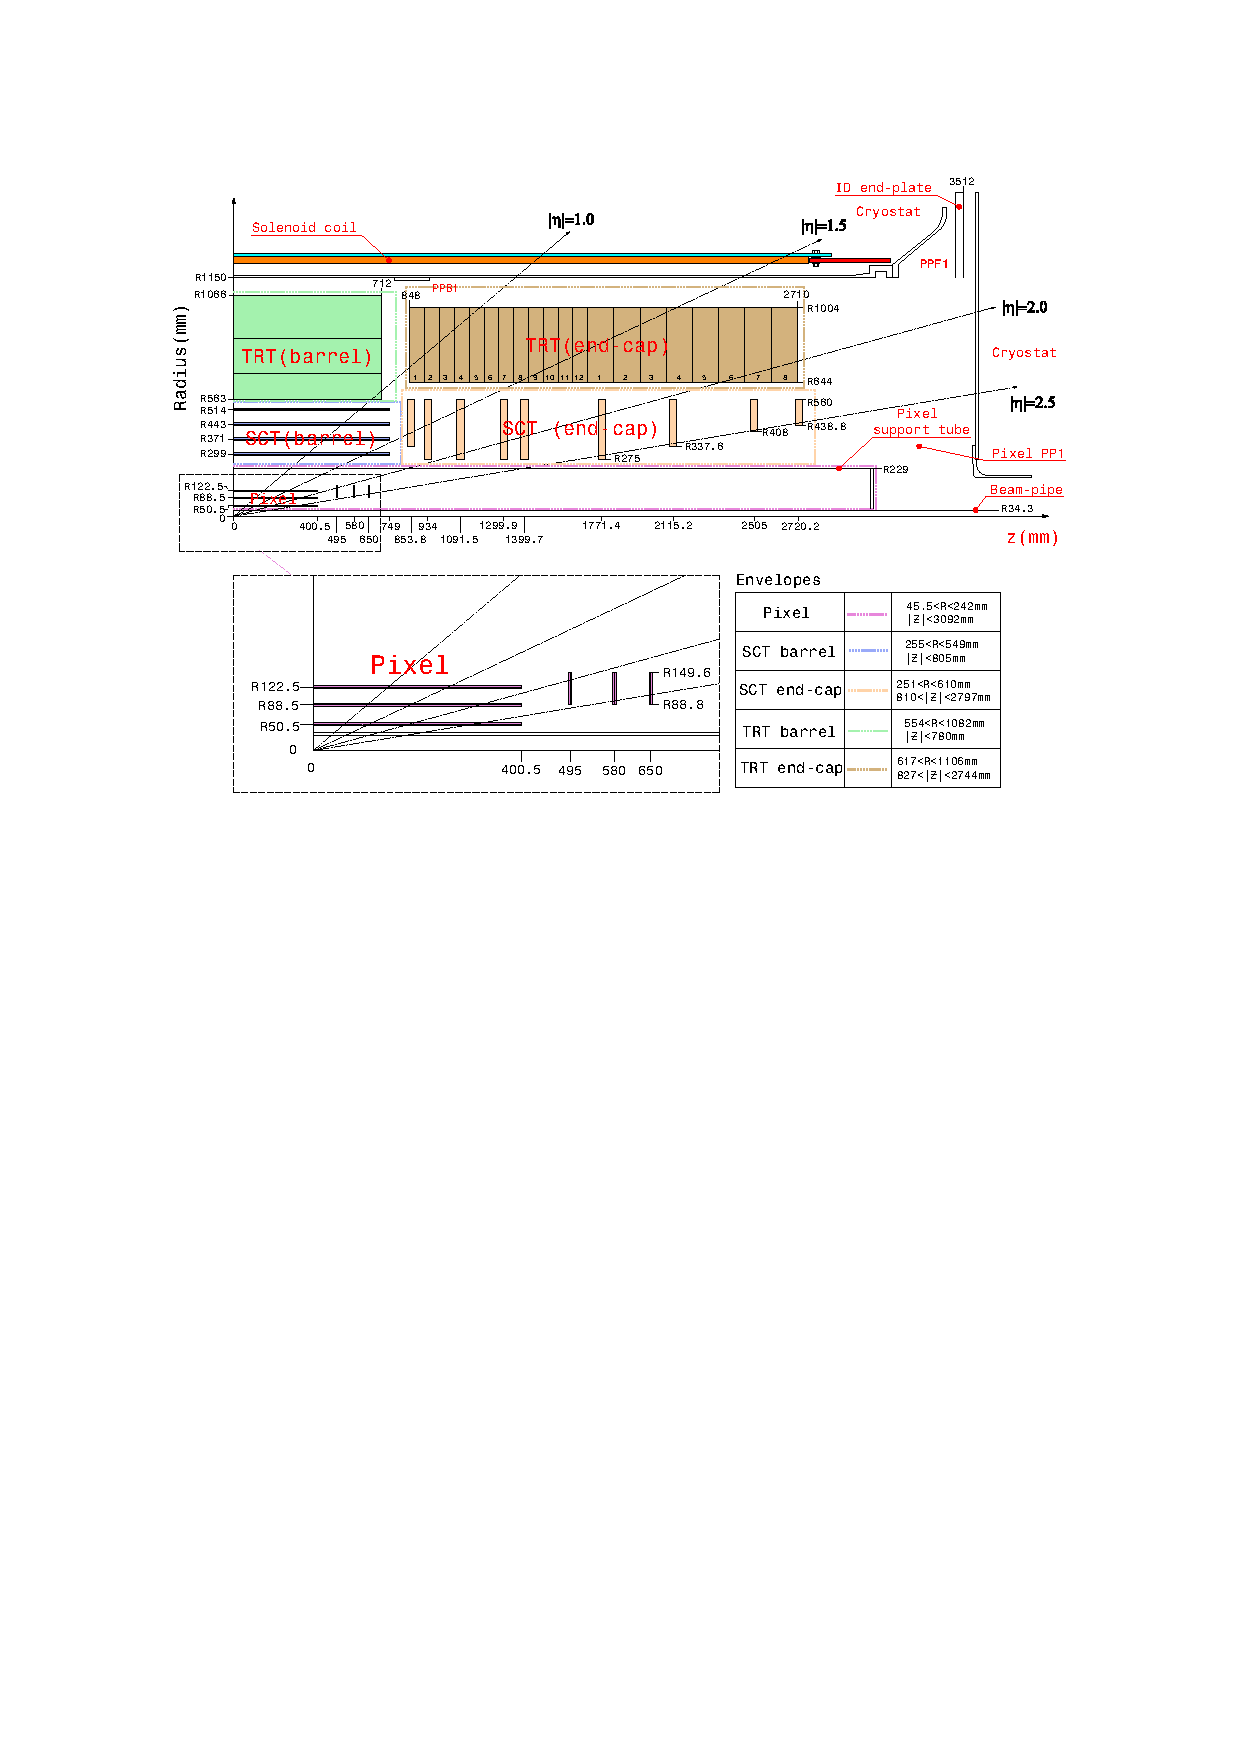
\includegraphics[width=.90\linewidth]{figures/atlas/ideta.pdf}
\caption{Diagram of one-quarter of the ATLAS Inner Detector, with lines drawn to indicate various $\eta$ locations. The labels PP1, PPB1 and PPF1 indicate the patch-panels for the ID services. TODO: what is that.}
\label{fig:IDeta}
\end{figure}
\end{centering}

\subsection{The Pixel Detector}

The Pixel detector lies closest to the beam pipe of the \ac{LHC}, and has four layers comprising 92 million read-out channels. There are three standard layers, referred to as Layers 1-3 (L1, L2, L3), and an additional layer added for the 2015 data-taking, called the \ac{IBL}. 

\subsubsection{The Original Pixel Detector}

The Pixel Detector consists of high-precision silicon chip pixel sensors, with 1744 sensors total. Each sensor is identical, containing 47232 pixels, which are typically each 50$\times$400 $\mu$m$^2$. 

As shown in \autoref{fig:IDeta}, the central $\eta$ region (barrel) is covered by three concentric cylindrical layers of sensors, while the higher $\eta$ region (endcap) is covered by a series of three disks positioned in the $x-y$ plane. Together, they give complete coverage out to $\eta = 2.5$, and a particle coming from the collision point will typically by measured by three layers. Each of these measurements is accurate in the barrel (endcap) to 10 $\mu$m in the $R-\phi$ direction and 115 $\mu$m in the $z$ ($R$) direction.  

\subsubsection{Addition of the IBL}

In 2015, the \ac{IBL} was lowered into the ATLAS cavern and added to the Pixel Detector. This layer sits on top of the beam pipe, inside barrel L1, which was formerly responsible for the first measurement of charged particles coming from a collision. 
TODO: add info about precision 


As the \ac{IBL}'s' name suggests, it was added to improve detection of $B$ mesons, whose non-trivial lifetimes create secondary vertices in ATLAS events, which allow them to be distinguished from other particles with precise track measurement. The \ac{IBL} is closer to the interaction point and has a smaller resolution, giving it a better chance to see these slightly displaced vertices.

\subsection{The Silicon Microstrip Tracker}

The \ac{SCT} employs similar technology to the Pixel Detector, with 15912 sensors and 6.3 million readout channels. Its difference from the Pixel Detector is in the readout, which is performed by a series of 12 cm long strips with a width of 80 $\mu$m. These layers are paired, placed on top of one another at a small (40 mrad) angle to allow for position determination in both directions, giving 4 spatial measurements for each particle passing through the \ac{SCT}. In the barrel, these strips run parallel to the beam pipe, while in the endcap, they are arranged radially. These strips have a resolution in the barrel (endcap) of 17 $\mu$m in the $R-\phi$ direction and 580 $\mu$m in the $z$ ($R$) direction. 

\subsection{The Transition Radiation Tracker}

The \ac{TRT} uses 4mm diameter gas-filled tubes, each with a high voltage wire suspended along the center of the tube. The tubes run the length of the barrel, with a separate wire in the positive and negative $z$ direction. In the endcap, the tubes are arranged radially. In total, there are about 351,000 readout channels in the \ac{TRT}. This detector makes measurements only in the $R-\phi$ direction, where the resolution of each measurement is 130 $\mu$m. Each particle typically creates about 36 hits as it passes through the \ac{TRT}. 

TODO is any of this right?
Particles passing through the gas mixture of the \ac{TRT} ionize the gas, producing electrons which drift towards the wire due to a potential difference applied between it and the straw. This process takes about 48 ns, and the signal can be directly read out, giving the fastest measurement of particles in the \ac{ID}. This speedy readout is essential to triggering, discussed more in \autoref{sec:Trigger}. 

The \ac{TRT} also responds to low-energy transition radiation photons, which produce a much larger signal than charged particles passing through the detector. Because of this strong difference in signals, hits from the \ac{TRT} are used to help differentiate between electrons and photons in the detector.

\section{The Calorimeters}
\label{sec:Calo}

Unlike the tracking detectors, which aim to take measurements of a particle with minimal alterations of its trajectory, the calorimeters measure the the energy of objects by stopping them entirely. The calorimeters, which can be seen in \autoref{fig:calo}, provide coverage out to $\eta$ < 4.9. Higher granularity electromagnetic measurements are made within $\eta$ < 2.5, where the \ac{ID} provides tracking capability, in order to give precision measurements of the energy of photons and electrons. The hadronic calorimeter provides coarser granularity, which is sufficient to determine the energy of jets. 

\begin{centering}
\begin{figure}[bth]
\myfloatalign
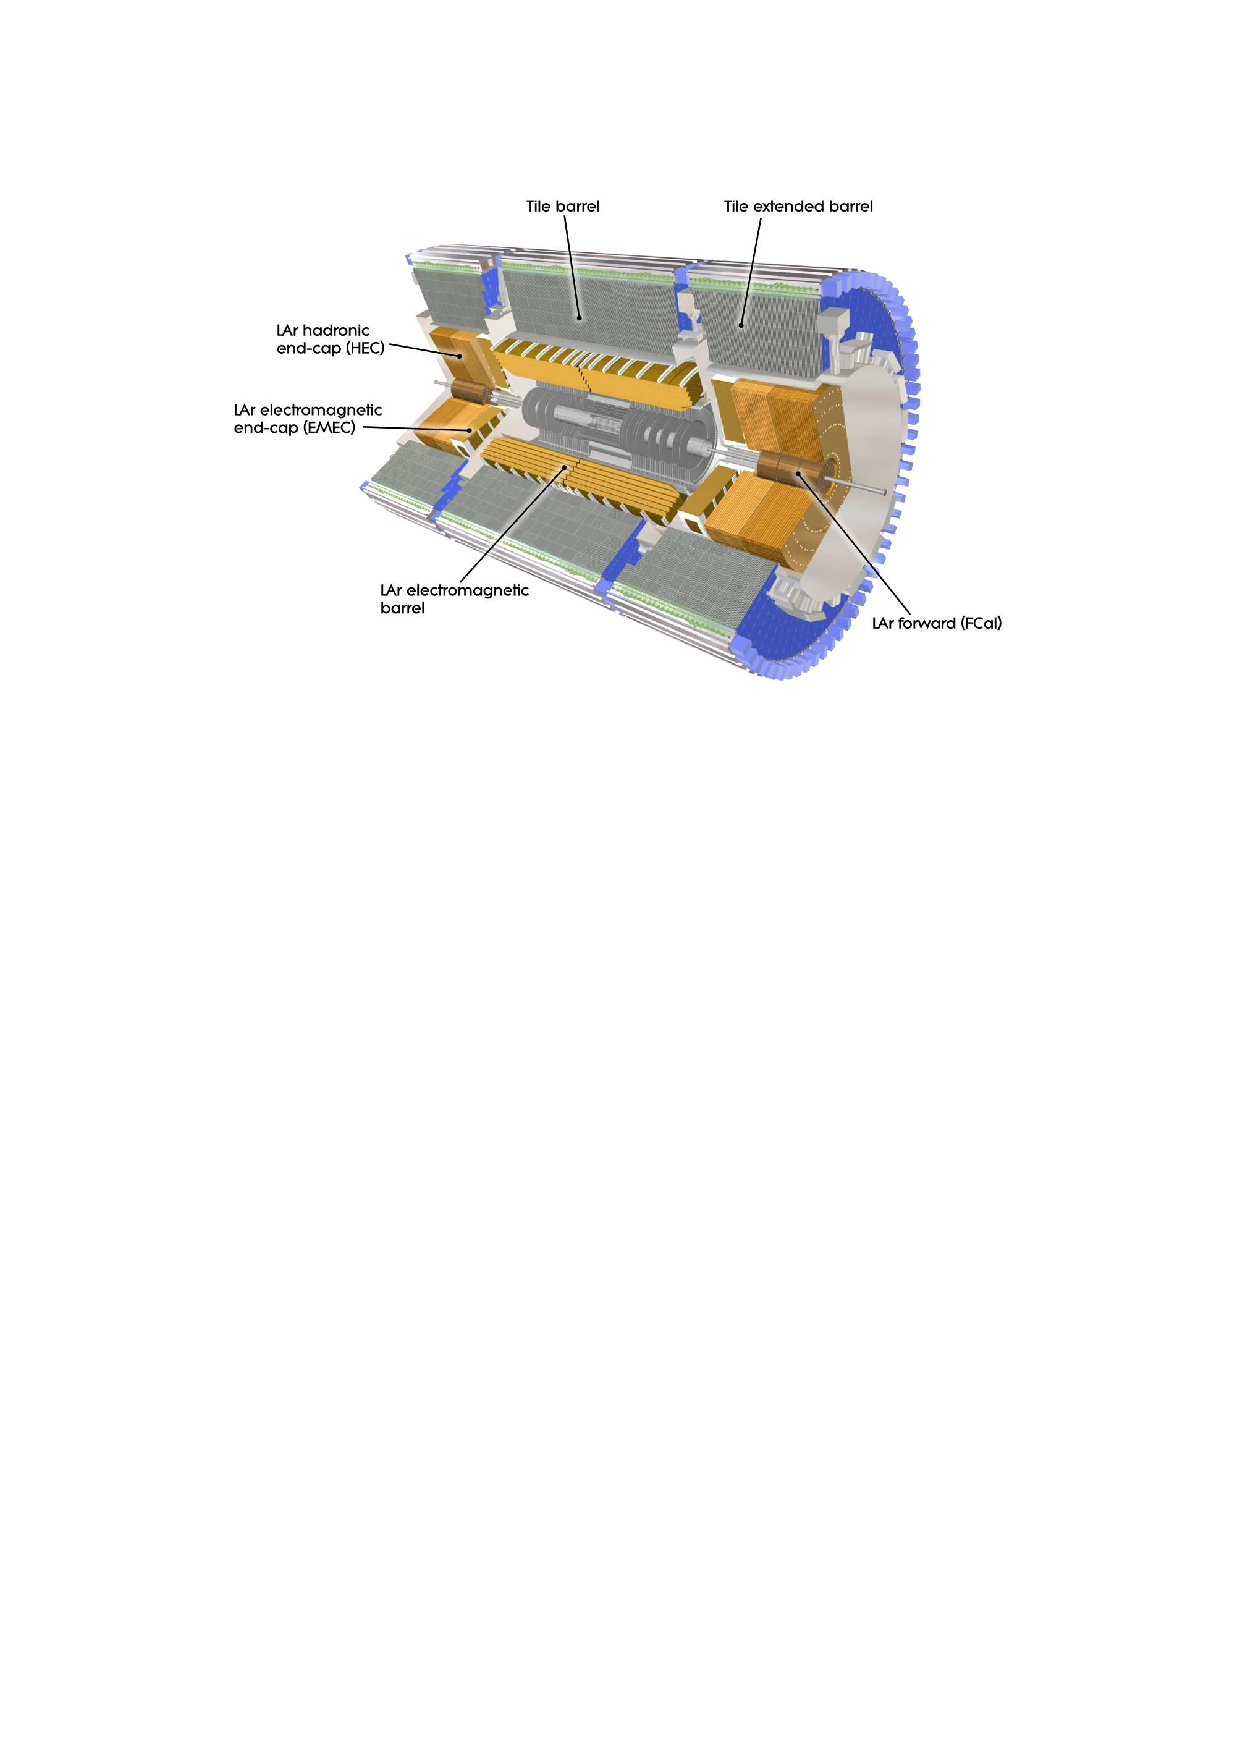
\includegraphics[width=.90\linewidth]{figures/atlas/calorimeters.pdf}
\caption{The calorimeter system of the ATLAS detector.}
\label{fig:calo}
\end{figure}
\end{centering}

TODO make sure jets are in theory.

Another task of the calorimeter system is to limit punch-through to the \ac{MS}, described in \autoref{sec:MS}. All other particles must be fully stopped by the calorimeters to allow for clean signals from muons, and to measure the total energy of the particle. This requirement sets minimum sizes for each of the calorimeters. 

\subsection{The LAr Electromagnetic Calorimeter}



\subsection{The Tile Calorimeter}

\section{The Muon Spectrometer}
\label{sec:MS}

\section{The Magnet System}

\section{The Trigger System}
\label{sec:Trigger}